\documentclass[pdftex,12pt,a4paper]{scrartcl}
\usepackage[english]{babel}
\usepackage{amsfonts}
\usepackage{amssymb}
\usepackage{physics}
\usepackage{amsmath}
\usepackage{xfrac}
\usepackage{graphicx}
\usepackage{caption}
\usepackage{subcaption}
\usepackage{placeins}
\usepackage{color}
\usepackage{nicefrac}
\newcommand\ddfrac[2]{\frac{\displaystyle #1}{\displaystyle #2}}
\newcommand{\opn}[1]{\operatorname{#1}}
\newcommand{\E}{\operatorname{E}}
\newcommand{\Var}{\operatorname{Var}}
\renewcommand{\P}{\mathbb{P}}


\begin{document}

The number of mutations $m$ found in a single cell after a time $t$ is given by the sum over all $u_i$ mutational events which occurred during each of its $y$ past divisions:
\begin{equation}
    m = \sum_i^{y} u_i
\end{equation}
Since division and mutation events are stochastic occurrences, $m$ is a random variable,
where the $u_i$ are Poisson distributen with identical rate $\mu$, and $y$ is taken Poisson distributed with rate $\lambda t$, so that $\lambda$ is an effective division rate.

\section{Symmetric divisions}

\subsection{Moran events}
Consider the case of only symmetric divisions: the daughter cells resulting from a division are either both differentiated (symmetric differentiation), or both remain stem cells (self-renewal). The former results in a loss of a cell from the population, while the latter leads to the addition of a new cell. Since the stem cell pool remains at fixed size the rates at which these two types of divisions occur must be equal: $\rho_{sym} = \rho_{sr} = \rho$ the rate of event occurrence \textit{per cell}. In a maximally stochastic model the occurences of self-renewals and differentiations would be independent processes (e.g. a classical birth-death process), however in such a system the size of the stem cell pool could vary stochastically. Since we are interested in a nonvarying stem cell pool, we opt for the minimally stochastic Moran model, which considers the limiting case of simultaneously occurring self-renewal and differentiation events. Applying the mutation burden distribution to the Moran model -- wherein we assume the Moran events (a simultaneous differentiation and self-renewal) occur in the pool as a Poisson process with rate $N\rho$ -- one might naively assume $\lambda = \rho$, given that $\lambda$ denotes the expected number of past divisions of a cell occurring in a unit time. We will however show that in a system with division occurring at a rate proportional to the size of the pool, the inclusion of cell removal (i.e. symmetric differentiation) results in $\lambda \approx 2\rho$.

\begin{figure}[h]
    \centering
    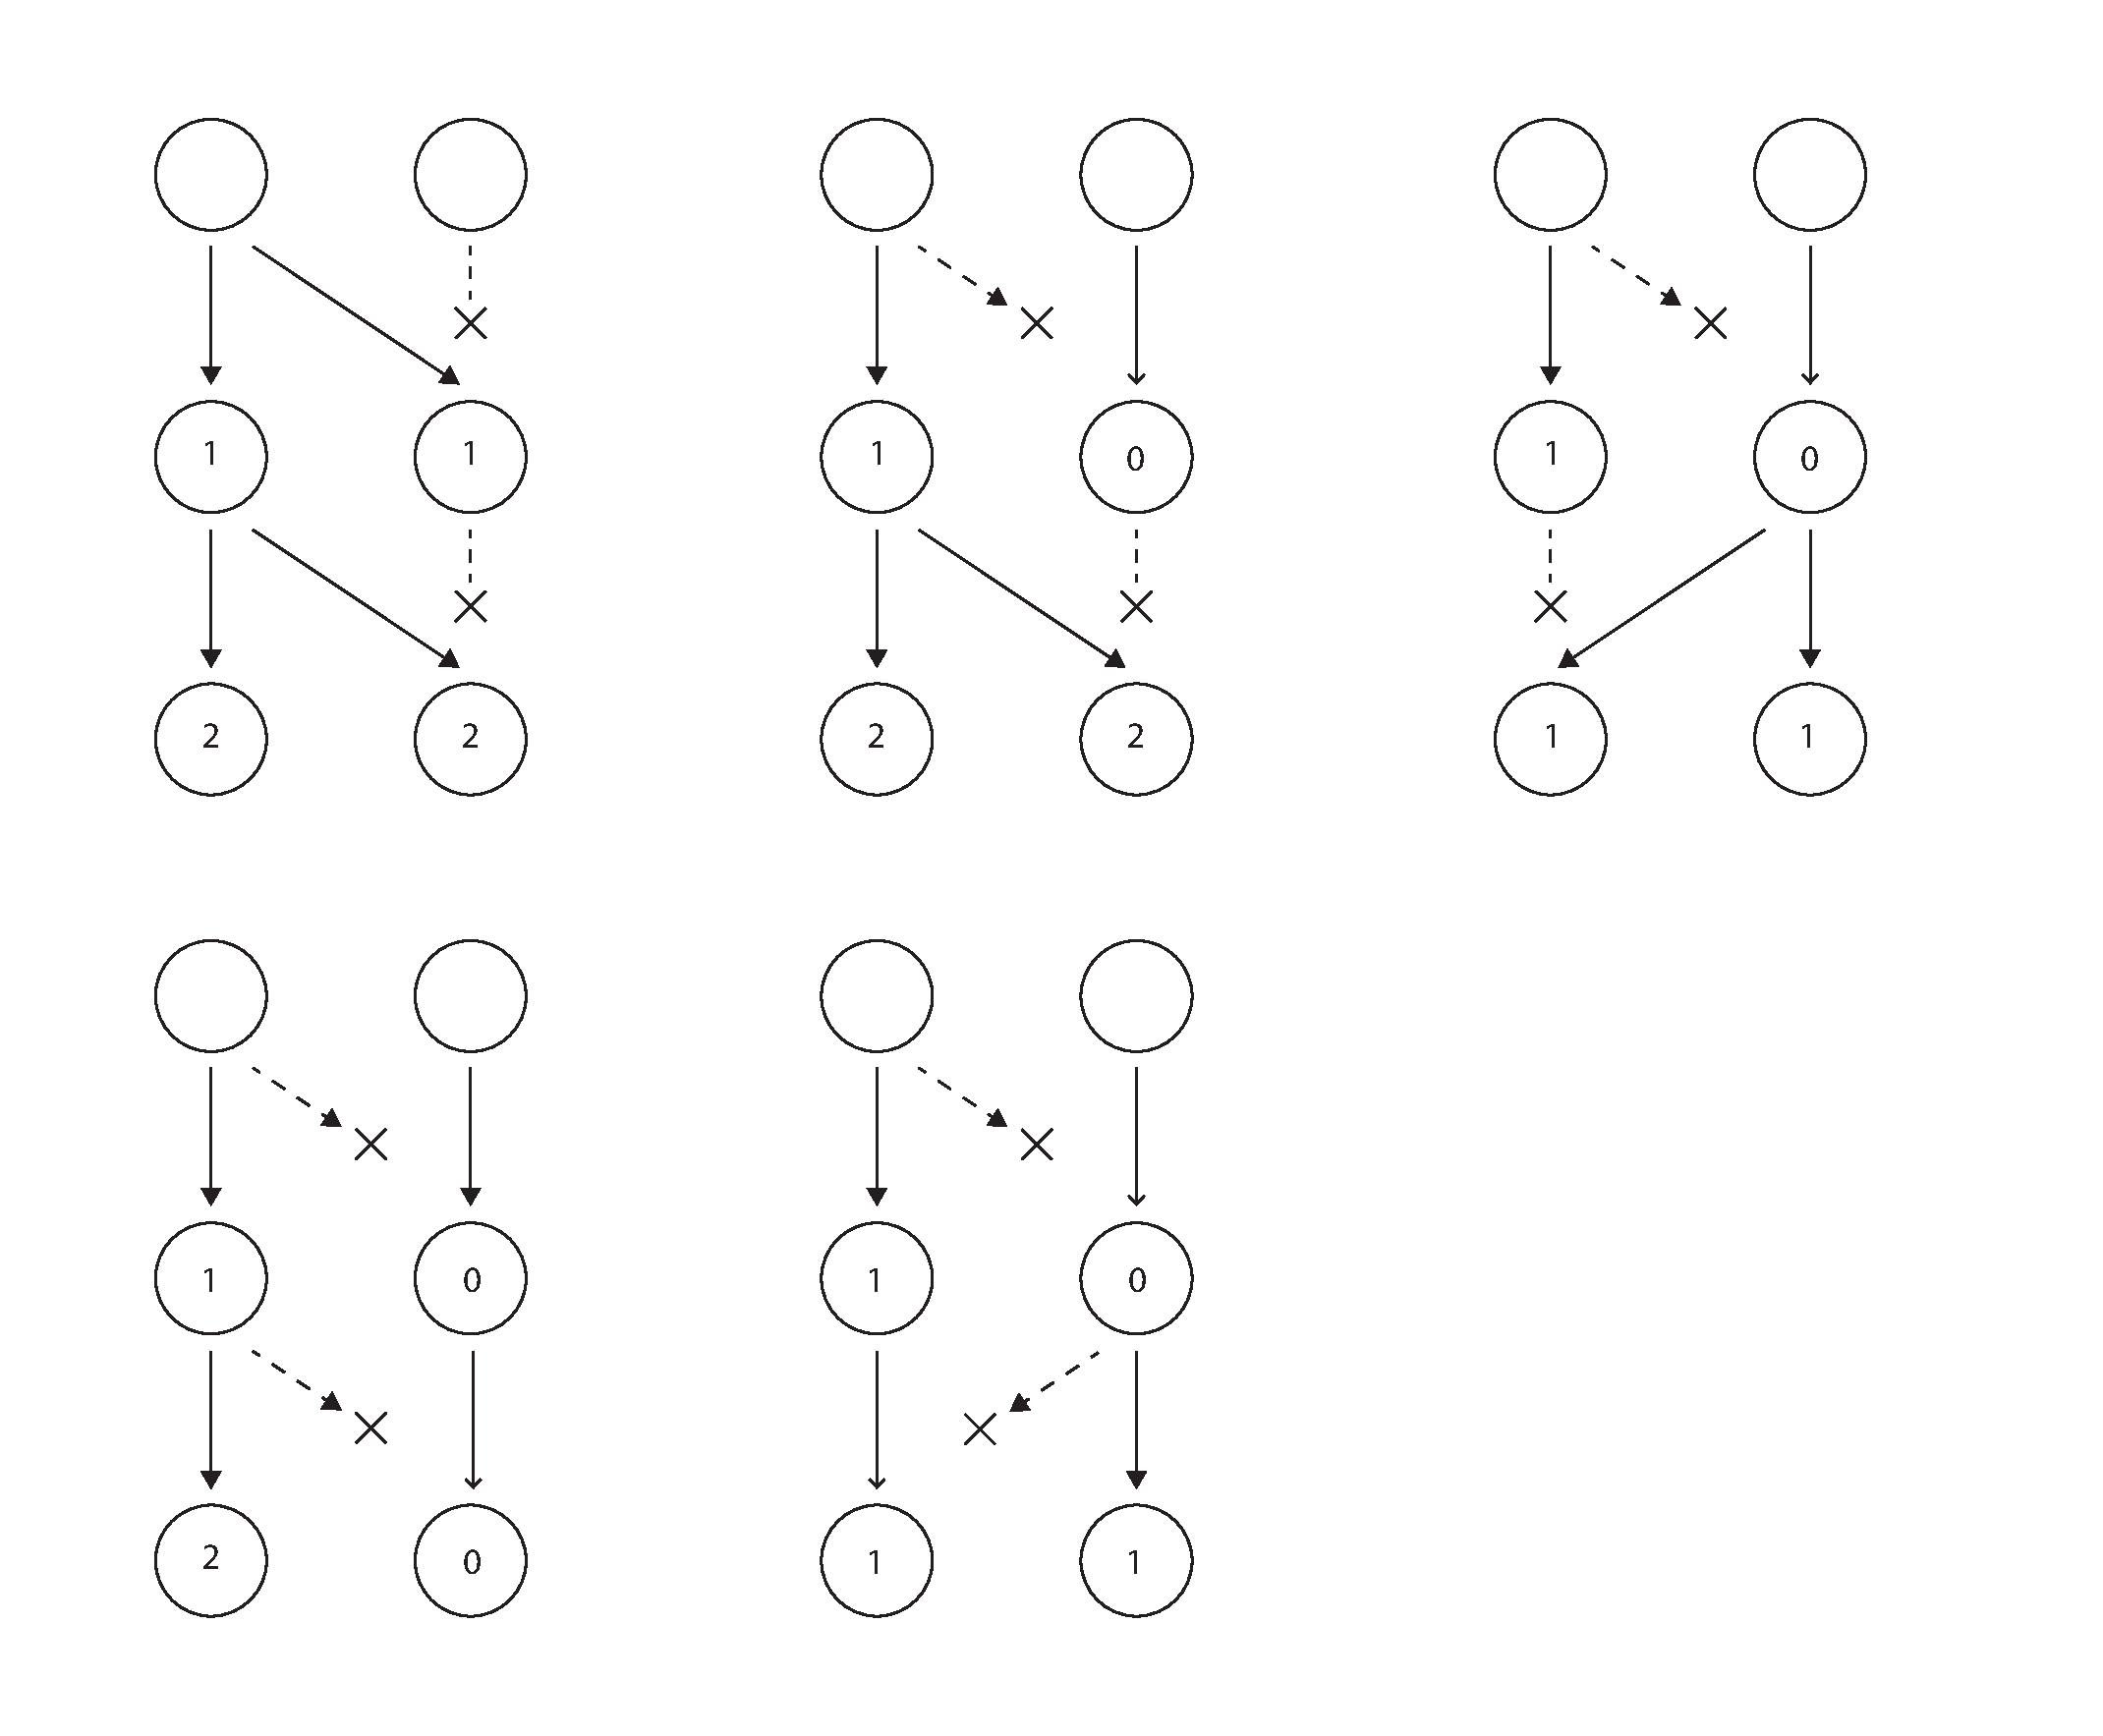
\includegraphics[width=\textwidth]{SCBurdenDivisionRate.pdf}
    \caption{...}
    \label{fig:N2divisions}
\end{figure}

Consider the simple system of two cells ($N=2$) which obey the Moran dynamics described above\footnote{Note that the result described here depends slightly on the precise definition of the Moran model, in particular, whether births and deaths are performed successively, with one occurring before the other, or simultaneously. Here we choose the model of simultaneous birth and death, where the same cell may be selected for both birth and death in a single event. If this occurs, the result is that one of the daughter cells is removed.}. The rate of event occurrences in the entire system is $N\rho$, and let us for simplicity take our time in units of $1/\rho$, meaning that we expect there on average to be 2 events occurring per unit time (one for each cell). If now we were to run the system for a single time unit -- say from time $t=0$ to $t=1$ and then observe it, $\lambda$ would denote the expected number of divisions that occurred for a single cell in this time, or in other words, the average number of past divisions across the two cells. Looking at the example scenario in Figure \ref{fig:N2divisions}, we see that for this realization of the stochastic process we end up with both cells having 2 divisions in their past history, which is equivalent to twice the per cell Moran rate $\rho$ (as our time step covered the expectation of 1 event per cell). Of course there might be other possible realizations of this system, and thus we are actually looking for the expected value over all possible evolutions. Fortunately, for this $N=2$ system these are quite easy to figure out, and we end up with $\lambda = (1+1/2)\rho$. Since this approach of considering the entire timestep is not particularly scalable to larger population sizes -- as the space of all possible outcomes grows combinatorially -- we note that the system is Markovian by construction (all events occur as Poisson processes, which by definition is memoryless), so that we need only calculate the expected $y'$ after the first event, and multiply this by the expected number of events in a timestep (which would be $N$) to obtain $\lambda$. For a single event, there are only two possible outcomes: either two different cells are selected for self-renewal and differentiation, or the same cell is selected for both. In the former case -- which occurs with probability $1-1/N$ -- the average number of divisions per cell is $2/N$; in the latter -- occurring with probability $1/N$ -- it is $1/N$. Thus after $N$ divisions (the expected number of divisions in the timestep) the expected number of divisions per cell is 
\begin{equation}
   y = N \qty[ \qty(1-\frac{1}{N})\frac{2}{N} + \frac{1}{N}\frac{1}{N} ] = 2 - 1/N
\end{equation}
and since we chose our timestep at $1/\rho$, we obtain for the effective division rate
\begin{equation}
    \lambda = \rho (2-1/N) \approx 2\rho
\end{equation}
with the final approximation obtained in the limit of large $N$.


\subsection{growth events}
Now what if a self-renewal is unaccompanied by a differentiation, i.e. in the case of an exponentially growing population? We can use exactly the same logic as above for a population of $N$ cells dividing at rate $\gamma$, though we must envision an infinitely short timespan, as the population size changes over time as well. After a single division, the average lineage length in the population is $2/(N(t)+1)$. Thus, with divisions occurring at rate $N(t)\gamma$ in the stem cell pool, after a infinitesimally short time $\tau$ the expected lineage length per cell is
\begin{equation}
    y(\tau) = N(t)\gamma \times 2/(N(t)+1) \times \tau = 2\gamma \frac{N(t)}{N(t)+1}\tau
\end{equation}



\section{Growing population}
Let us now consider the case of a growing population with asymmetric divisions at rate $\phi$, symmetric Moran divisions (which are the simulaneous self-renewal and differentiation events described above) at rate $\rho$, and self-renewal divisions which contribute to population growth at rate $\gamma$. The expected number of divisions per lineage after a time $t$ is then given by
\begin{equation}
    y(t) = \int_0^t \qty[ 2\rho \qty(1 - \frac{1}{2N(\tau)} ) + \phi + 2\gamma \qty(1 - \frac{1}{N(\tau)+1}) ] d\tau
\end{equation} 

\end{document}